%% 
%% Copyright 2019-2024 Elsevier Ltd
%% 
%% This file is part of the 'CAS Bundle'.
%% --------------------------------------
%% 
%% It may be distributed under the conditions of the LaTeX Project Public
%% License, either version 1.3c of this license or (at your option) any
%% later version.  The latest version of this license is in
%%    http://www.latex-project.org/lppl.txt
%% and version 1.3c or later is part of all distributions of LaTeX
%% version 1999/12/01 or later.
%% 
%% The list of all files belonging to the 'CAS Bundle' is
%% given in the file `manifest.txt'.
%% 
%% Template article for cas-sc documentclass for 
%% double column output.

\documentclass[a4paper,fleqn]{cas-sc}

% If the frontmatter runs over more than one page
% use the longmktitle option.

%\documentclass[a4paper,fleqn,longmktitle]{cas-sc}

%\usepackage[numbers]{natbib}
%\usepackage[authoryear]{natbib}
\usepackage[authoryear,longnamesfirst]{natbib}

\usepackage{algorithm}
\usepackage[noend]{algorithmic}
\usepackage{subcaption}
\usepackage{enumitem}

%%%Author macros
\usepackage{amssymb}
\usepackage{xspace}

\newcommand{\even}          {\raisebox{0.3ex}{\scalebox{0.7}{$\bigcirc$}}\xspace}
\newcommand{\odd}           {\scalebox{0.9}{$\square$}\xspace}
\newcommand{\subeven}       {\raisebox{0.3ex}{\scalebox{0.5}{$\bigcirc$}}\xspace}
\newcommand{\subodd}        {\scalebox{0.6}{$\square$}\xspace}
\newcommand{\player}        {\mathsf{p}\xspace}
\newcommand{\opponent}      {\overline{\mathsf{p}}\xspace}

\newcommand{\wregularform}  {$\omega$-regular form\xspace}
\newcommand{\wregulargames} {$\omega$-regular games\xspace}
\newcommand{\noc}           {{\small\textsf{No\textit{-}Opponent\textit{-}Cycle}}\xspace}
\newcommand{\nocchecker}    {{\small\textsf{NOC\textit{-}Checker}}\xspace}
\newcommand{\noceager}      {{\small\textsf{NOC\textit{-}Eager}}\xspace}
\newcommand{\nocfilter}     {{\small\textsf{NOC\textit{-}Filter}}\xspace}
\newcommand{\nocmemo}       {{\small\textsf{NOC\textit{-}Memo}}\xspace}
\newcommand{\nocq}          {{\small\textsf{NOCQ}}\xspace}
\newcommand{\zra}           {{\small\textsf{ZRA}}\xspace}

% \newtheorem{definition}{Definition}
% \newtheorem{example}{Example}

% % Define MiniZinc syntax highlighting
% \lstdefinelanguage{MiniZinc}{
%   keywords={include, constraint, output, array, of, var, bool},
%   morekeywords={[2] set, int, float, string},
%   keywordstyle=\color{blue}\bfseries,
%   keywordstyle={[2]\color{teal}\bfseries},
%   sensitive=true,
%   comment=[l]{\%}, 
%   morecomment=[s]{/*}{*/},
%   commentstyle=\color{gray}\ttfamily,
%   stringstyle=\color{red}\ttfamily,
%   morestring=[b]",    % Defines double-quoted strings
%   morestring=[b]',    % Defines single-quoted strings  basicstyle=\ttfamily\small,
%   numberstyle=\tiny\color{gray},
%   numbers=left,
%   stepnumber=1,
%   breaklines=true,
%   showstringspaces=false,
%   frame=single,
%   tabsize=2,
%   basicstyle=\ttfamily\footnotesize
% }

% \lstset{
%     basicstyle=\small\ttfamily,
%     backgroundcolor=\color{gray!10},
%     frame=single,
%     framerule=0pt,
%     columns=fullflexible,
%     breaklines=true,
%     xleftmargin=0.5em,
%     xrightmargin=0.5em
% }
\def\tsc#1{\csdef{#1}{\textsc{\lowercase{#1}}\xspace}}
\tsc{WGM}
\tsc{QE}
%%%

% Uncomment and use as if needed
%\newtheorem{theorem}{Theorem}
%\newtheorem{lemma}[theorem]{Lemma}
%\newdefinition{rmk}{Remark}
%\newproof{pf}{Proof}
%\newproof{pot}{Proof of Theorem \ref{thm}}

\begin{document}
\let\WriteBookmarks\relax
\def\floatpagepagefraction{1}
\def\textpagefraction{.001}

% Short title
\shorttitle{}    

% Short author
\shortauthors{}  

% Main title of the paper
\title [mode = title]{Constraint base approach for solving deterministic \wregulargames}  

% Title footnote mark
% eg: \tnotemark[1]
\tnotemark[1] 

% Title footnote 1.
% eg: \tnotetext[1]{Title footnote text}
\tnotetext[1]{Chalo} 

% First author
%
% Options: Use if required
% eg: \author[1,3]{Author Name}[type=editor,
%       style=chinese,
%       auid=000,
%       bioid=1,
%       prefix=Sir,
%       orcid=0000-0000-0000-0000,
%       facebook=<facebook id>,
%       twitter=<twitter id>,
%       linkedin=<linkedin id>,
%       gplus=<gplus id>]

\author[1]{}%[<options>]

% Corresponding author indication
\cormark[1]

% Footnote of the first author
\fnmark[1]

% Email id of the first author
\ead{}

% URL of the first author
\ead[url]{}

% Credit authorship
% eg: \credit{Conceptualization of this study, Methodology, Software}
\credit{}

% Address/affiliation
\affiliation[1]{organization={},
            addressline={}, 
            city={},
%          citysep={}, % Uncomment if no comma needed between city and postcode
            postcode={}, 
            state={},
            country={}}

\author[2]{}%[]

% Footnote of the second author
\fnmark[2]

% Email id of the second author
\ead{}

% URL of the second author
\ead[url]{}

% Credit authorship
\credit{}

% Address/affiliation
\affiliation[2]{organization={},
            addressline={}, 
            city={},
%          citysep={}, % Uncomment if no comma needed between city and postcode
            postcode={}, 
            state={},
            country={}}

% Corresponding author text
\cortext[1]{Corresponding author}

% Footnote text
\fntext[1]{}

% For a title note without a number/mark
%\nonumnote{}

% Here goes the abstract
\begin{abstract}
Solving \wregulargames is a core problem in formal verification, particularly within model checking and synthesis methods that have several industrial-scale applications. In this paper, we propose a constraint-based approach for games on graphs, built upon a novel propagation algorithm that eliminates opponent cycles from the game graph. This approach yields an efficient method that directly exploits the duality between players in a parity game. Our implementation within a Lazy Clause Generation framework outperforms all existing constraint-based methods for parity games. Furthermore, it performs competitively against the most specialized, non-CP-based algorithms---often matching and sometimes exceeding their performance---while retaining the inherent flexibility of general constraint-based approaches. 

Because new constraints can be seamlessly integrated, our method provides a highly flexible framework for refining existing problem formulations to search for preferred solutions. This extensibility allows the framework to solve multi-conditioned games, such as those combining parity conditions with cost or resource-bounded requirements. Finally, we present the theoretical foundations of our approach, a comprehensive experimental evaluation, and an analysis of different algorithmic variants.
\end{abstract}

% Use if graphical abstract is present
%\begin{graphicalabstract}
%\includegraphics{}
%\end{graphicalabstract}

% Research highlights
\begin{highlights}
\item 
\item 
\item 
\end{highlights}


% Keywords
% Each keyword is seperated by \sep
\begin{keywords}
Constraint programming  \sep Parity games \sep Verification.
\end{keywords}

\maketitle

\section{Introduction}
Two-player, zero-sum, infinite-duration games played on graphs provide the foundational mathematical framework for the automated verification and synthesis of reactive systems. In this paradigm, vertices represent states of the system and its environment, edges denote possible transitions or actions, and infinite paths (plays) represent the ongoing behavior of the system. Solving these games—determining which player can force a play to satisfy a specific objective—is central to model checking, synthesis of controllers, and verifying specifications against adversarial environments.
%
Depending on the system requirements, these objectives are specified using different winning conditions on infinite paths. These are broadly categorized into qualitative and quantitative conditions. Qualitative conditions focus on the structural or topological properties of infinite paths; classic examples include Büchi conditions (visiting designated states infinitely often), Rabin conditions, and parity conditions (evaluating the parity of the maximum priority seen infinitely often). Quantitative conditions, on the other hand, incorporate resource constraints or performance metrics, such as energy conditions (keeping a running resource counter above zero) and mean-payoff conditions (optimizing the long-run average reward).
%
While specialized, highly tuned algorithms exist for isolated game types—most notably for parity games, which belong to $\mathsf{NP} \cap \mathsf{co\textit{-}NP}$~\cite{Jurdziński:1998}  —handling multi-conditioned objectives or transitioning between qualitative and quantitative variants often requires abandoning the underlying algorithmic machinery entirely. Because these state-of-the-art approaches rely on dedicated engines hardcoded to exploit the distinct mathematical structure of a single winning condition, they lack architectural modularity. Consequently, extending them to multi-conditioned settings typically requires complex reductions that fundamentally alter the game graph, leading to severe state-space explosion.
%
Traditional attempts to apply general combinatorial optimization frameworks, such as static reductions to Boolean Satisfiability (SAT), suffer from severe scalability bottlenecks. Forbidding winning cycles for an opponent via propositional logic leads to a massive explosion in formula size~\cite{Heljanko:2012}, severely limiting their practical application. In this paper, we overcome these limitations by presenting a unified, constraint-based approach capable of solving deterministic \wregulargames across a spectrum of winning conditions. Instead of relying on rigid, monolithic encodings, our approach is built upon a novel propagation algorithm designed to dynamically eliminate opponent winning cycles from the game graph. By abstracting the core graph reasoning into a dedicated constraint propagator, our method directly exploits the inherent duality between players, providing a symmetric and highly efficient mechanism for filtering invalid actions.
%
We implement this system within a Lazy Clause Generation (LCG) framework~\cite{DBLP:journals/constraints/OhrimenkoSC09}. By dynamically reasoning about the graph's structure during search and generating precise explanations for edge prunings, our framework combines the operational efficiency of specialized graph algorithms with the conflict-driven learning capabilities of modern constraint solvers. Empirical evaluations \cite{Hernandez:2026:noc} demonstrate that this approach not only outperforms previous constraint-based and SAT-based formulations for qualitative games like parity, but also performs highly competitively against state-of-the-art, non-CP-based specialized algorithms. More importantly, we show that the inherent flexibility of general constraint programming allows our framework to seamlessly scale from purely qualitative objectives (Büchi, Rabin, parity) to complex quantitative settings (energy, mean-payoff), as well as multi-conditioned formulations where qualitative and quantitative constraints must be satisfied simultaneously.

The remainder of this paper is organized as follows. Section...

\section{Preliminaries}\label{sec:prelims}

\subsection{Turn-Based Games on Graphs}
\label{subsec:turn_based_games}

An \wregulargame is a two-player, zero-sum game of infinite duration played on a directed graph called an \textit{arena}. Two players, \textit{Even} (denoted as $\even$ or $0$) and \textit{Odd} (denoted as $\odd$ or $1$), move a token along adjacent vertices. The vertex where the token currently resides determines which player chooses the next transition. This ongoing process generates an infinite sequence of states. The ultimate winner of the game depends on whether this sequence satisfies a specific objective, defined by the game's winning condition.

\begin{definition}[Arena]\label{def:arena}
A turn-based game \textit{arena} $\mathcal{A}$ is a tuple $\mathcal{A} = (V, E, \Omega, Q)$, where:
\begin{itemize}
    \item $V$ is a finite set of vertices partitioned into two disjoint sets: $V_{\even}$ (vertices controlled by Player~$\even$) and $V_{\odd}$ (vertices controlled by Player~$\odd$).
    \item $E \subseteq V \times V$ is a set of directed transitions such that every vertex has at least one outgoing edge, i.e., $\forall v \in V, |vE| \geq 1$, where $vE = \{ w \in V \mid (v, w) \in E \}$ denotes the set of successors of $v$. We denote $Ev = \{ u \in V \mid (u, v) \in E \}$ as the set of predecessors of $v$.
    \item $\Omega: V \to \mathbb{N}$ is a priority coloring function that assigns to each vertex a non-negative integer priority (primarily utilized in qualitative and parity contexts).
    \item $Q: E \to \mathbb{Z}$ is a weight function that assigns an integer weight to each transition, representing resource costs or rewards (primarily utilized in quantitative contexts).
\end{itemize}
\end{definition}

A game begins with a token placed at an initial vertex $v_0 \in V$. If $v_0 \in V_{\even}$, Player~$\even$ selects a successor $v_1 \in v_0E$; if $v_0 \in V_{\odd}$, Player~$\odd$ makes the selection. The token is then moved to $v_1$, and the process repeats indefinitely. This sequence of choices produces an infinite path $\pi = v_0 v_1 v_2 \ldots$ such that $(v_i, v_{i+1}) \in E$ for all $i \geq 0$, which is formally termed a \textit{play}. We denote the set of all infinite plays in $\mathcal{A}$ as $\text{Plays}(\mathcal{A})$. Given a play $\pi$, we define $\text{Inf}(\pi) \subseteq V$ as the set of vertices that appear infinitely often in $\pi$.

\subsection*{Strategies and Determinism}
% A \textit{strategy} for a player is a recipe specifying which successor to choose based on the history of the play up to the current vertex. In this work, we focus on \textit{memoryless} (or positional) strategies, which are sufficient for solving the standard classes of deterministic $\omega$-regular games considered here. A memoryless strategy for Player~$\even$ is a function $\sigma: V_{\even} \to V$ such that $\sigma(v) \in vE$ for all $v \in V_{\even}$. Symmetrically, a memoryless strategy for Player~$\odd$ is a function $\tau: V_{\odd} \to V$ such that $\tau(v) \in vE$ for all $v \in V_{\odd}$. 

% A profile consisting of a pair of memoryless strategies $(\sigma, \tau)$ completely determines a unique play $\pi(v_0, \sigma, \tau) = v_0 v_1 v_2 \ldots$ starting from any initial vertex $v_0$, where $v_{i+1} = \sigma(v_i)$ if $v_i \in V_{\even}$ and $v_{i+1} = \tau(v_i)$ if $v_i \in V_{\odd}$. 

% An objective $\mathcal{W}$ for Player~$\even$ is a subset of all possible infinite plays, $\mathcal{W} \subseteq \text{Plays}(\mathcal{A})$. A play $\pi$ is winning for Player~$\even$ if $\pi \in \mathcal{W}$; otherwise, because the games are zero-sum, the play is winning for Player~$\odd$. A strategy $\sigma$ is a winning strategy for Player~$\even$ from a vertex $v_0$ if for all possible strategies $\tau$ of the opponent, the resulting play $\pi(v_0, \sigma, \tau)$ belongs to $\mathcal{W}$. Solving a game means partitioning the vertex set $V$ into two winning regions $W_{\even}$ and $W_{\odd}$, containing the vertices from which Player~$\even$ and Player~$\odd$ possess a winning strategy, respectively.


% \subsection*{Strategies and Initial-Vertex Game Solving}
A \textit{memoryless} strategy for Player~$\even$ is a function $\sigma: V_{\even} \to V$ such that $\sigma(v) \in vE$ for all $v \in V_{\even}$. Symmetrically, a memoryless strategy for Player~$\odd$ is a function $\tau: V_{\odd} \to V$ such that $\tau(v) \in vE$ for all $v \in V_{\odd}$. These strategies depend solely on the current position of the token, ignoring the history of the play. A pair of memoryless strategies $(\sigma, \tau)$ completely determines a unique infinite play $\pi(v_0, \sigma, \tau) = v_0 v_1 v_2 \ldots$ starting from a designated initial vertex $v_0 \in V$. 

An objective $\mathcal{W}$ for Player~$\even$ is a subset of all possible infinite plays, $\mathcal{W} \subseteq \text{Plays}(\mathcal{A})$. A strategy $\sigma$ is a winning strategy for Player~$\even$ from the initial vertex $v_0$ if, for all possible adversarial strategies $\tau$ of Player~$\odd$, the resulting unique play satisfies the objective, i.e., $\pi(v_0, \sigma, \tau) \in \mathcal{W}$. Due to the memoryless determinism of the deterministic \wregulargames\ studied here~\cite{Zielonka:1998}, if a player has a winning strategy from $v_0$, they are guaranteed to have a memoryless one. 

In this work, we focus on the \textit{initial-vertex game solving problem}. Given a game arena $\mathcal{A}$ and a specific starting vertex $v_0 \in V$, the goal is to determine which of the two players has a winning strategy starting from $v_0$, and to construct that specific winning strategy.

\subsection{Winning Conditions for \wregulargames}
\label{subsec:winning_conditions}

The classification of an infinite play as winning or losing is governed by the game's \textit{winning condition}, which dictates how the path's structural or numerical properties are evaluated. From a player's perspective, this condition defines their \textit{objective} $\mathcal{W} \subseteq \text{Plays}(\mathcal{A})$, representing the specific set of plays they aim to enforce. For consistency across all discussed variants, we focus on the objective $\mathcal{W}$ from the perspective of Player~$\even$. Because these games are zero-sum, a play $\pi$ is winning for Player~$\even$ if $\pi \in \mathcal{W}$, and winning for Player~$\odd$ if $\pi \notin \mathcal{W}$. 

We partition these objectives into two major paradigms: \textit{qualitative conditions}, which evaluate the structural topology of the vertices visited infinitely often, and \textit{quantitative conditions}, which evaluate the numerical accumulation of resource weights along the traversed edges.

\subsubsection{Qualitative Conditions}
\label{subsubsec:qualitative}

Qualitative conditions depend strictly on the set of vertices that appear infinitely often in a play $\pi$, denoted as $\text{Inf}(\pi) \subseteq V$.

\paragraph{Büchi and co-Büchi Objectives:}
A Büchi condition is defined relative to a designated set of target vertices $F \subseteq V$. The objective for Player~$\even$ is to visit this set infinitely often. Formally, a play $\pi$ satisfies the Büchi objective if:
\[
\text{Inf}(\pi) \cap F \neq \emptyset
\]
Conversely, the dual co-Büchi objective requires that the play eventually settles outside the complement of $F$, meaning that vertices outside of $F$ are visited only finitely many times. A play $\pi$ satisfies the co-Büchi objective if $\text{Inf}(\pi) \subseteq F$.

\paragraph{Rabin and Streett Objectives:}
A Rabin condition is parameterized by a finite collection of pairs $R = \{(E_1, F_1), (E_2, F_2), \ldots, (E_k, F_k)\}$, where $E_j, F_j \subseteq V$ for each $j \in \{1, \ldots, k\}$. Player~$\even$ wins the Rabin objective if there exists at least one index $j$ where the play visits $E_j$ infinitely often but $F_j$ only finitely often:
\[
\exists j \in \{1, \ldots, k\} \text{ such that } \text{Inf}(\pi) \cap E_j \neq \emptyset \text{ and } \text{Inf}(\pi) \cap F_j = \emptyset
\]
The Streett condition is the deterministic complement of the Rabin condition. It requires that for every index $j$, if the set $E_j$ is visited infinitely often, then the set $F_j$ must also be visited infinitely often:
\[
\forall j \in \{1, \ldots, k\}, \quad \text{Inf}(\pi) \cap E_j \neq \emptyset \implies \text{Inf}(\pi) \cap F_j \neq \emptyset
\]

\paragraph{Parity Objectives:}
The parity condition evaluates a play using the arena's priority coloring function $\Omega: V \to \mathbb{N}$. Player~$\even$ satisfies the parity objective if the maximum priority that appears infinitely often along the play is an even integer:
\[
\max \{ \Omega(v) \mid v \in \text{Inf}(\pi) \} \bmod 2 = 0
\]
If the maximum infinite priority is odd, the play is won by Player~$\odd$.


\subsubsection{Quantitative Conditions}
\label{subsubsec:quantitative}

Quantitative conditions shift the evaluation to the infinite sequence of transitions $e_0 e_1 e_2 \ldots$ generated during a play $\pi = v_0 v_1 v_2 \ldots$, tracking numerical behaviors via the arena's edge weight function $Q: E \to \mathbb{Z}$.

\paragraph{Energy Objectives:}
Energy conditions model games with physical resource constraints (such as fuel, electricity, or memory). Given an initial resource capacity $c_{\text{init}} \in \mathbb{N}$ and an upper storage boundary $W \in \mathbb{N} \cup \{\infty\}$, the energy level $c_k$ after $k$ transitions is tracked dynamically via the recurrence relation $c_{k+1} = \min(W, c_k + Q(e_k))$, where $c_0 = c_{\text{init}}$. Player~$\even$ wins the energy objective if the running resource total remains non-negative at every step along the infinite play:
\[
\forall k \geq 0, \quad c_k \geq 0
\]

\paragraph{Mean-Payoff Objectives:}
The mean-payoff condition evaluates the long-term average reward or cost accumulated per transition. The numerical value assigned to a play $\pi$ is defined as the limit inferior of the average edge weights over time:
\[
\mu(\pi) = \liminf_{n \to \infty} \frac{1}{n} \sum_{i=0}^{n-1} Q(e_i)
\]
Given a target performance threshold $\nu \in \mathbb{R}$, Player~$\even$ satisfies the mean-payoff objective if the long-run average meet or exceeds this bound:
\[
\mu(\pi) \geq \nu
\]


% \section{Constraint Programming Framework for Game Solving}\label{sec:cp_framework}
% \subsection{Decision Variables and Local Strategy Characterization}\label{subsec:variables_local}
% \subsection{Baseline Formulation: Monolithic SAT Encoding}\label{subsec:sat_baseline}

\section{Constraint Programming Framework for Game Solving}
\label{sec:cp_framework}

This section describes our constraint programming (CP) framework for solving deterministic \wregulargames\ from an initial-vertex perspective. We first formalize how local memoryless strategies are characterized via Boolean decision variables. We then outline the traditional monolithic SAT/SMT baseline formulation to highlight the structural and scalability challenges that motivate our unified global propagator approach.

% =========================================================================
% SUBSECTION 3.1: DECISION VARIABLES AND LOCAL STRATEGY CHARACTERIZATION
% =========================================================================
\subsection{Decision Variables and Local Strategy Characterization}
\label{subsec:variables_local}

To solve an initial-vertex game using a constraint-based approach, the search space for a winning memoryless strategy must be mapped into finite-domain decision variables. Let $\player \in \{\even, \odd\}$ denote the \textit{player of interest}, and let $\opponent = 1 - \player$ represent their designated opponent. We partition the finite set of vertices $V$ of the arena $\mathcal{A}$ into $V_{\player}$ (vertices controlled by the player of interest) and $V_{\opponent}$ (vertices controlled by the opponent). 

Given a specific starting vertex $v_0 \in V$, we introduce two sets of Boolean decision variables to track the active sub-graph induced by the players' strategic choices during the search:
\begin{itemize}
    \item $\mathcal{V}_v \in \{\top, \bot\}$ for each vertex $v \in V$, denoting whether vertex $v$ is reachable from $v_0$ under the currently explored strategy profile.
    \item $\mathcal{E}_e \in \{\top, \bot\}$ for each directed edge $e \in E$, denoting whether transition $e$ is actively selected or traversed within the strategy sub-graph.
\end{itemize}

The structural conditions required to characterize a valid winning region from $v_0$ for the player of interest are deeply rooted in the classic game-theoretic concept of an \textit{attractor}~\cite{Zielonka:1998,Aggarwal:2023}. Given a target set of vertices, the $\player$-attractor is the set of states from which $\player$ can force the play into that target set in a finite number of steps, regardless of the choices made by $\opponent$. 

To embed this operational capability natively into our CP variable framework, the active strategy sub-graph must be constrained such that $\player$ maintains absolute deterministic control, while simultaneously guarding against every possible counter-move from $\opponent$. Structurally, this requires enforcing the following connectivity rules from $v_0$:
\begin{enumerate}
    \item \textbf{Root Activation:} The initial vertex must always be active ($\mathcal{V}_{v_0} = \top$).
    \item \textbf{Deterministic Selection:} For every active vertex controlled by the player of interest ($v \in V_{\player}$), the solver must select at least one outgoing transition to enforce a positional choice.
    \item \textbf{Adversarial Closure:} For every active vertex controlled by the opponent ($v \in V_{\opponent}$), the formulation must activate \textit{all} of its outgoing transitions. This models the attractor logic by guaranteeing that no matter which edge the opponent selects, the play cannot escape the verified strategy graph.
    \item \textbf{Forward Propagation:} Any vertex reached by an active edge must itself be marked as active.
\end{enumerate}

By combining these structural layout constraints, the CP solver isolates a well-formed sub-arena where Player~$\player$ has a valid strategy from $v_0$. The remaining task for the solver is to ensure that the cycles formed within this attractor structure satisfy the designated qualitative or quantitative winning conditions.


---

% =========================================================================
% SUBSECTION 3.2: BASELINE FORMULATION AND EXTENSION TO GENERAL CSP
% =========================================================================
\subsection{Baseline Formulations and the Generalized CSP Model}
\label{subsec:sat_baseline}

Historically, constraint-based game solving has relied on encoding cycle conditions statically into propositional logic. The standard reference approach by Heljanko et al.~\cite{Heljanko:2012} translates a game into Boolean Satisfiability (SAT) or Satisfiability Modulo Theories (SMT) formulas by leveraging a \textit{progress measure}~\cite{Jurdziński:2000}.

In this baseline formulation, the structural graph properties are captured by the following Conjunctive Normal Form (CNF) clauses:
\begin{itemize}
    \item $\Phi_\exists = \bigwedge_{v \in V_{\subeven}} \left(S_v \rightarrow \bigvee_{w \in vE} T_{(v,w)}\right)$
    \item $\Phi_\forall = \bigwedge_{v \in V_{\subodd}} \left(S_v \rightarrow \bigwedge_{w \in vE} T_{(v,w)}\right)$
    \item $\Phi_V = \bigwedge_{w \in V, w \neq v_0} \left( \left(\bigvee_{v \in Ev} T_{(v,w)}\right) \rightarrow S_w \right)$
\end{itemize}
where $S_v$ and $T_{(v,w)}$ are Boolean variables tracking the winning paths for Player~$\even$. 
%
To enforce the parity condition along infinite paths, additional integer variables $x_p^v$ are introduced for every vertex $v$ and every odd priority $p \in \textit{Odd}(G)$. These variables track numerical progress along active transitions via difference logic constraints ($\Phi_A$):


To enforce the parity condition along infinite paths, additional integer variables $x_p^v$ are introduced for every vertex $v \in V$ and every odd priority $p \in \textit{Odd}(G)$, where $\textit{Odd}(G) = \{ p \in \mathbb{N} \mid p \pmod 2 \neq 0 \land \exists v \in V: \Omega(v) = p \}$ represents the set of all odd priorities present in the arena. These variables track numerical progress along active transitions via difference logic constraints ($\Phi_A$):

\begin{itemize}
    \item $\Phi_A = \bigwedge_{(v,w) \in E} \left(T_{(v,w)} \rightarrow \Psi_{(v,w)}\right)$
    \item $\Psi_{(v,w)} = \bigwedge_{p \in \textit{Odd}^{>\Omega(w)}(G)} (x_p^v \geqslant x_p^w), \quad \text{if } \Omega(w) \text{ is even}$
    \item $\Psi_{(v,w)} = \bigwedge_{p \in \textit{Odd}^{>\Omega(w)}(G)} (x_p^v \geqslant x_p^w) \land (x_{\Omega(w)}^v > x_{\Omega(w)}^w), \quad \text{if } \Omega(w) \text{ is odd}$
\end{itemize}
These difference logic assertions force a strict mathematical contradiction (such as $x_p^v > x_p^v$) along any active cycle dominated by an odd priority. This renders the system of constraints logically unsatisfiable along that specific path, structurally forcing the solver's backtracking engine to reject assignments containing odd-winning loops and isolate only even-winning cycles.

The fundamental principle of this constraint-based approach is to reduce game-theoretic determinacy to propositional satisfiability. Determining the satisfiability of the combined formula $(S_{v_0} \wedge \Phi_{\exists} \wedge \Phi_{\forall} \wedge \Phi_V \wedge \Phi_A)$ is equivalent to deciding the winner of the game. A satisfying assignment serves as a constructive proof that Player~\even\ has a winning strategy from $v_0$. Conversely, because the encoding completely characterizes Player~\even's winning conditions, an exhaustive proof of unsatisfiability establishes that no such strategy exists, which—by the determinacy of these games—constitutes a definitive proof of a win for Player~\odd.

\subsubsection{Limitations of the Monolithic Baseline}
While highly effective for pure parity games on small arenas, this monolithic encoding faces severe scaling and architectural bottlenecks when generalized to broader $\omega$-regular contexts:
\begin{enumerate}
     \item \textbf{Space and Formula Explosion:} In terms of static allocation space, the method requires instantiating $\mathcal{O}(|V| \cdot |\textit{Odd}(G)|)$ auxiliary variables and generating $\mathcal{O}(|E| \cdot |\textit{Odd}(G)|)$ difference logic constraints. For dense graphs with rich priority profiles, this upfront space requirement grows up to $\mathcal{O}(|V|^3)$. Crucially, this footprint escalates even further when the formulation is reduced to pure SAT solving. Converting the underlying integer difference logic into pure CNF requires bit-blasting or explicit circuit encodings for every inequality, multiplying the clause count and injecting hundreds of millions of literal allocations before the search even begins.
    \item \textbf{Inflexibility to Multi-Objectives:} Adapting progress measures to quantitative metrics (like energy levels or long-run averages) requires fundamentally reconstructing the underlying arithmetic variable layers, destroying the modularity of the framework.
\end{enumerate}

To overcome these structural limitations, we replace the entire monolithic CNF formula—including both the static graph connectivity clauses and the progress measure variables—with a unified, high-level Constraint Satisfaction Problem (CSP) abstraction. Instead of flattening the game's rules into a rigid propositional grid, this CP model captures the graph's topology natively through clean domain variables, while seamlessly handling arbitrary, multi-conditioned $\omega$-regular properties by delegating all cycle validation to a dynamic global propagator.

\begin{definition}[Generalized Game CSP]\label{def:csp}
The CSP for an arena $\mathcal{A} = (V, E, \Omega, Q)$ starting at an initial vertex $v_0$ from the perspective of Player~$\player$ is defined as the triple $\mathcal{P} = (\mathcal{X}, \mathcal{D}, \mathcal{C})$, where $\mathcal{X} = \{ \mathcal{V}_v \}_{v \in V} \cup \{ \mathcal{E}_e \}_{e \in E}$ represents the set of Boolean decision variables mapped to domains $\mathcal{D} = \{\bot, \top\}$, and $\mathcal{C}$ is the set of constraints defined by:
\begin{itemize}
    [leftmargin=2.3cm, labelwidth=2.8cm, align=right, itemsep=1.0ex, parsep=0pt]
    \item [$\mathcal{C}_{v_0}$ :] $\mathcal{V}_{v_0} = \top$
    \item [$\mathcal{C}_{\player}$ :] $\bigwedge_{v \in V_{\player}} \left(\mathcal{V}_v \rightarrow \left(\sum_{w \in vE} \mathcal{E}_{(v,w)}= 1\right)\right)$
    \item [$\mathcal{C}_{\opponent}$ :] $\bigwedge_{v \in V_{\opponent}} \left(\mathcal{V}_v \rightarrow \bigwedge_{w \in vE} \mathcal{E}_{(v,w)}\right)$
    \item [$\mathcal{C}_{\!E}$ :] $\bigwedge_{w \in V, w \neq v_0} \left(\left(\bigvee_{v \in Ew} \mathcal{E}_{(v,w)}\right) \rightarrow \mathcal{V}_w\right)$
    \item [$\mathcal{C}_{\!N\!O\!C}(f)$ :] $\bigwedge_{v_0, \closerdots, v_k} \left( \left(\bigwedge_{i=0}^{k-1} \mathcal{E}_{(v_i,v_{i+1})}\right) \to \bigwedge_{j=0}^{k-1} \left((v_j = v_k) \to f(v_j, \closerdots, v_k)\right) \right)$
\end{itemize}
where the evaluation criteria $f$ for a given cycle $v_j, \dots, v_k$ are provided by specific qualitative or quantitative verification functions—encompassing Büchi ($f^B$), Rabin ($f^R$), Parity ($f^\omega$), Energy ($f^\eta$), and Mean-Payoff ($f^\mu$) conditions—which are formally detailed in Section~\ref{sec:function_conditions}.

\end{definition}

While constraints $\mathcal{C}_{v_0}$, $\mathcal{C}_{\opponent}$, and $\mathcal{C}_{\!E}$ enforce the required sub-graph connectivity (analogous to the baseline's $\Phi_{v_0}, \Phi_\forall$, and $\Phi_V$), $\mathcal{C}_{\player}$ strictly dictates that the protagonist selects exactly one deterministic strategy choice per active vertex. 

Crucially, our approach removes the expensive difference logic constraints $\Phi_A$ entirely. Instead, the global constraint $\mathcal{C}_{\!N\!O\!C}(f)$ monitors the strategy graph dynamically during the CP search loop. It intercepts any emerging path profile and applies a parameterized verification function $f$ to ensure that any reachable closed component is structurally or quantitatively winning for $\player$. The precise operational formulations for these qualitative and quantitative cycle evaluation functions are detailed thoroughly in Section~\ref{sec:function_conditions}.

Our generalized CSP model inherits and extends this satisfiability approach, lifting it from a fixed perspective to a modular framework. The semantic mapping between the satisfiability of the CSP and the game-theoretic outcome remains definitive: a satisfying assignment found by the solver proves that the player of interest, $\player$, possesses a positional winning strategy from $v_0$, where the active edges ($\mathcal{E}_e = \top$) map directly to their winning choices. 

A key architectural advantage of this design is that by simply swapping the roles of $\player$ and $\opponent$, the formulation allows the proposed method to search from the perspective of either player natively. While a satisfying assignment validates a win for $\player$, an exhaustive proof of unsatisfiability demonstrates the complete absence of a positional winning strategy for them, which—by the determinacy of these games—automatically hands a conclusive victory to the opponent $\opponent$.

\subsection{Running Example}
\label{subsec:running_example}

\begin{figure}
     \centering
     % Pull the images slightly into the margins to maximize center space
     \makebox[\textwidth][c]{
         \begin{subfigure}[t]{0.51\textwidth}
             \centering
             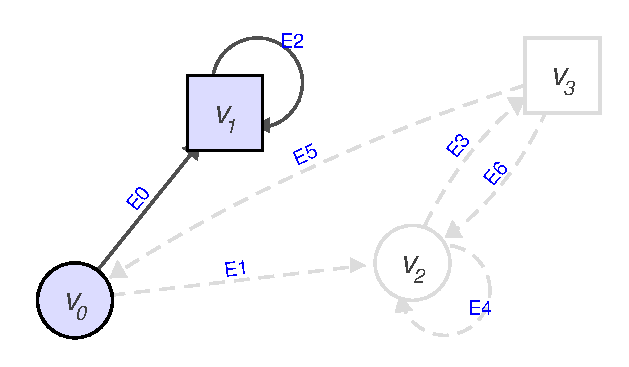
\includegraphics[width=0.8\textwidth, trim={0 0 0 0}, clip]{images/ex01.pdf}
             \vspace{-5pt} % Reduces gap between image and sub-caption
             \caption{First assignment.}
             \label{fig:ex01}
         \end{subfigure}
         \hspace{1pt} % Minimal gap
         \begin{subfigure}[t]{0.51\textwidth}
             \centering
             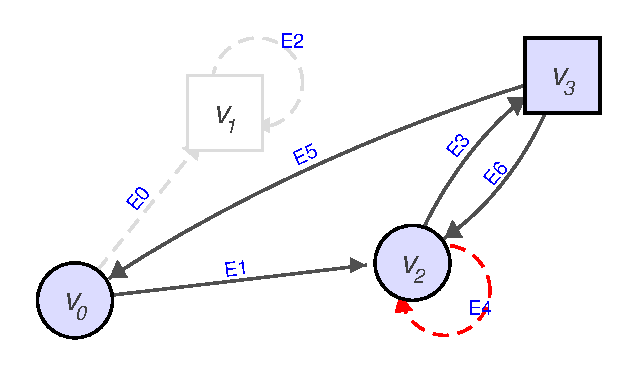
\includegraphics[width=0.8\textwidth, trim={0 0 0 0}, clip]{images/ex02.pdf}
             \vspace{-5pt}
             \caption{Second assignment}
             \label{fig:ex02}
         \end{subfigure}
     }
     \caption{Arena with 4 vertices and 6 edges.  Vertices controlled by Player \even are shown as circles, while vertices controlled by Player \odd are shown as squares.}
     \label{fig:ex00}
\end{figure}

To demonstrate the structural and operational mechanics of our generalized CSP formulation, consider the 2-player game arena illustrated in Figure~\ref{fig:ex00}. The arena consists of four vertices $V = \{v_0, v_1, v_2, v_3\}$, which are partitioned into $V_{\subeven} = \{v_0, v_1\}$ (represented as circles) and $V_{\subodd} = \{v_2, v_3\}$ (represented as squares). The directed edge set is defined as $E = \{e_0, e_1, e_2, e_3, e_4, e_5\}$. We evaluate a Büchi objective from the perspective of Player~$\even$ ($\player = \even$), where the target accepting set is $F = \{v_1\}$, and the initial vertex is $v_0$.

Under our framework, the solver instantiates the core set of Boolean decision variables:
\[
\mathcal{X} = \{\mathcal{V}_0, \mathcal{V}_1, \mathcal{V}_2, \mathcal{V}_3, \mathcal{E}_0, \mathcal{E}_1, \mathcal{E}_2, \mathcal{E}_3, \mathcal{E}_4, \mathcal{E}_5\}
\]
mapped to individual Boolean domains $\mathcal{D}$. The structural and global constraints execute through the following progression:

\begin{enumerate}
    \item \textbf{Root Activation ($\mathcal{C}_{v_0}$):} The search initializes by anchoring the root vertex: $\mathcal{V}_0 = \top$.
    \item \textbf{Deterministic Strategy Choice ($\mathcal{C}_{\player}$):} Vertex $v_0$ is controlled by Player~$\even$. The constraint forces exactly one outgoing edge to be selected. 
    \begin{itemize}
        \item If the solver branches and tests $\mathcal{E}_0 = \top$, forward propagation ($\mathcal{C}_E$) activates vertex $v_3$ ($\mathcal{V}_3 = \top$). Because vertex $v_3$ belongs to Player~$\odd$, its outgoing edge is forced active ($\mathcal{E}_5 = \top$), closing a localized cycle on vertex $v_3$ (See Figure \ref{fig:ex01}). The global constraint evaluates $f^B(v_3, v_3) = \{v_3\} \cap \{v_1\} \neq \emptyset$, which returns $\bot$. The propagator immediately rejects this branch, forcing the solver to backtrack.
        \item The solver then selects the winning alternative: $\mathcal{E}_1 = \top$. This choice propagates and activates vertex $v_1$ ($\mathcal{V}_1 = \top$).
    \end{itemize}
    \item \textbf{Propagation Loop:} At vertex $v_1$, Player~$\even$ must again pick exactly one deterministic transition. The solver selects $\mathcal{E}_2 = \top$, which propagates and activates the opponent's vertex $v_2$ ($\mathcal{V}_2 = \top$).
    \item \textbf{Attractor Logic Realization ($\mathcal{C}_{\opponent}$):} Because vertex $v_2$ is controlled by the opponent, constraint $\mathcal{C}_{\opponent}$ triggers. To guarantee that Player~$\even$ is safe against any adversarial counter-play, the model forces \textit{all} outgoing transitions from vertex $v_2$ to activate simultaneously:
    \[
    \mathcal{V}_2 \rightarrow (\mathcal{E}_3 \land \mathcal{E}_4)
    \]
    Consequently, both $\mathcal{E}_3$ and $\mathcal{E}_4$ are set to $\top$ (See Figure \ref{fig:ex02}).
\end{enumerate}

At this stage, the structural layout constraints have successfully isolated a candidate strategy sub-graph. The global constraint $\mathcal{C}_{\!N\!O\!C}(f^B)$ now scans this active sub-arena and extracts all reachable cycles resulting from the opponent's split at vertex $v_2$:
\begin{itemize}
    \item \textbf{Cycle 1 ($v_0 \rightarrow v_1 \rightarrow v_2 \rightarrow v_0$):} Traversing edges $e_1, e_2, e_4$, the solver evaluates the cycle sequence:
    \[
    f^B(v_0, v_1, v_2, v_0) = \{v_0, v_1, v_2\} \cap \{v_1\} \neq \emptyset \implies \top
    \]
    \item \textbf{Cycle 2 ($v_1 \rightarrow v_2 \rightarrow v_1$):} Reachable via $e_0$ and traversing edges $e_2, e_3$, the solver evaluates the tighter loop:
    \[
    f^B(v_1, v_2, v_1) = \{v_1, v_2\} \cap \{v_1\} \neq \emptyset \implies \top
    \]
\end{itemize}

Because every active cycle within this adversarial attractor structure satisfies the function $f^B$, the global constraint validates the assignment. The solver successfully terminates, outputting a satisfying strategy assignment proving that Player~$\even$ wins the game from $v_0$.



\subsection{Global Opponent Cycle Elimination Propagators}
\label{sec:global_propagators}

Before detailing the inner workings of our cycle elimination algorithms, it is important to clarify how the different components of the generalized Game CSP (Definition~\ref{def:csp}) are implemented within the underlying solver. The localized structural constraints—namely the root activation ($\mathcal{C}_{v_0}$), the player's deterministic choice ($\mathcal{C}_{\player}$), the opponent's attractor expansion ($\mathcal{C}_{\opponent}$), and the forward edge propagation ($\mathcal{C}_E$)—consist of simple, local logical dependencies. Consequently, they are mapped directly to standard propositional clauses or native primitive constraints managed efficiently by the solver's default propagation engine. 

In contrast, the cycle validation constraint $\mathcal{C}_{\!N\!O\!C}(f)$ governs non-local, dynamic graph properties that cannot be captured effectively by static clauses. This necessitates the introduction of a custom, highly specialized global propagator to monitor the emerging strategy graph and dynamically prune illegal loops during search.

To dynamically enforce the global constraint $\mathcal{C}_{\!N\!O\!C}(f)$ during the search loop, we introduce three algorithmic variants designed to intercept, analyze, and eliminate illegal winning components for the opponent $\opponent$. Rather than relying on rigid, upfront propositional expansions, these propagators run natively inside the CP solver's execution engine, providing varying trade-offs between filtering strength and algorithmic complexity.


Before detailing the inner workings of our cycle elimination algorithms, it is important to clarify how the different components of the generalized Game CSP (Definition~\ref{def:csp}) are implemented within the underlying solver. The localized structural constraints—namely the root activation ($\mathcal{C}_{v_0}$), the player's deterministic choice ($\mathcal{C}_{\player}$), the opponent's attractor expansion ($\mathcal{C}_{\opponent}$), and the forward edge propagation ($\mathcal{C}_E$)—consist of simple, local logical dependencies. Consequently, they are mapped directly to standard propositional clauses or native primitive constraints managed efficiently by the solver's default propagation engine. 

In contrast, the cycle validation constraint $\mathcal{C}_{\!N\!O\!C}(f)$ governs non-local, dynamic graph properties that cannot be captured effectively by static clauses. This necessitates the introduction of a custom, highly specialized global propagator to monitor the emerging strategy graph and dynamically prune illegal loops during search.

To make this global propagator fully modular across multi-conditioned arenas, we decouple the global path evaluation function $f$ into an abstract, vertex-level winning predicate. We define the global objective profile as a conjunctive operator composition over the individual game criteria:
\[
f = f^B \otimes f^R \otimes f^\omega \otimes f^\eta \otimes f^\mu 
\]
where $B, R, \omega, \eta$, and $\mu$ represent qualitative and quantitative objectives (specifically Büchi, Rabin, parity, energy boundaries, and mean-payoffs, respectively). 

Correspondingly, for any individual state, the predicate $f_{\player}(v)$ evaluates whether the local property of vertex $v$ satisfies or actively contributes to the winning requirements of $\player$ under the composed objective $f_{\player}$. If $f_{\player}(v)$ holds true, vertex $v$ belongs to the safe region for the player of interest; if false ($\neg f_{\player}(v)$), the state inherently risks driving the game into a component dominated by the adversary. The algorithms in this section leverage this predicate to systematically slice away valid sub-graphs and isolate losing loops.

\subsubsection{A No-Opponent-Cycle Checker (NOCChecker)} \label{sec:nocchecker}

Our first baseline propagator establishes a fundamental validation check by recursively decomposing the strategy sub-graph into Strongly Connected Components (SCCs). By definition, every vertex inside an SCC of cardinality greater than one belongs to at least one localized cycle, whereas single-vertex SCCs can only close a loop via an explicit self-loop. 

The checker isolates the induced active sub-graph containing only assigned variables where $\mathcal{V}_v = \top$ and $\mathcal{E}_e = \top$. It then systematically identifies and eliminates vertices that satisfy the winning condition for $\player$, checking whether any residual components form an inescapable cycle that exclusively favors $\opponent$.

\begin{algorithm}[htb]
\small
\caption{\textbf{\textit{NOCChecker}}}
\textbf{Input}: Induced active sub-graph $G = (V', E')$ \\
\textbf{Output}: $\top$ if the strategy graph contains no winning opponent cycles; $\bot$ otherwise
\begin{algorithmic}[1]
    \FOR{$scc \in \textit{Tarjan}(G)$} \label{alg:noc-checker:breakingdown}
        \IF{$|scc| = 1$} \label{alg:noc-checker:single}
            \STATE $v \gets$ the unique vertex in $scc$
            \STATE \textbf{if } $\neg f_{\player}(v) \land \mathcal{E}_{[vEv]}$ \textbf{then return $\bot$} \label{alg:noc-checker:self}  
        \ELSE
            \STATE $ \textit{objectiveSet} \gets \{ v \in scc \mid 
            f_{\player}(v) \text{ holds true}
            \}$ \label{alg:noc-checker:best}
            \STATE \textbf{if } $ \textit{objectiveSet} = \emptyset$ \textbf{then return $\bot$} \label{alg:noc-checker:opponent}

            \STATE \textit{NOCChecker}($G \setminus \textit{objectiveSet}$) \label{alg:noc-checker:recursion}
        \ENDIF
    \ENDFOR
    \RETURN $\top$
\end{algorithmic}
\label{alg:noc-checker}
\end{algorithm}

Algorithm~\ref{alg:noc-checker} is executed when all decision variables within the current search branch become fixed. The function is invoked with the induced sub-graph containing exclusively the active components: $\textit{NOCChecker}(\{ v \in V \mid \mathcal{V}_v = \top \})$.

The graph is first partitioned into independent components using Tarjan's linear-time algorithm (Line~\ref{alg:noc-checker:breakingdown}). If an SCC contains an isolated vertex (Line~\ref{alg:noc-checker:single}), the algorithm ensures it does not possess an active self-loop ($\mathcal{E}_{[vEv]} = \top$) that violates the evaluation predicate $f_{\player}(v)$ (Line~\ref{alg:noc-checker:self}). For non-trivial components, the algorithm isolates the subset of vertices that satisfy the winning criteria for the player of interest: $\textit{objectiveSet} \gets \{ v \in scc \mid f_{\player}(v) \}$ (Line~\ref{alg:noc-checker:best}). 

If this filtering step yields an empty set ($\textit{objectiveSet} = \emptyset$), it mathematically demonstrates that the entire component forms a closed cycle where no state can satisfy the winning criteria for $\player$ (Line~\ref{alg:noc-checker:opponent}). Due to the structural nature of these games, this represents an inescapable loop favoring the adversary, and the assignment is rejected. Otherwise, if the set is not empty, those validated states are filtered out, and the checker is recursively called on the remaining induced sub-graph ($G \setminus \textit{objectiveSet}$) to ensure that no secondary, losing sub-cycles are nested within the component (Line~\ref{alg:noc-checker:recursion}).

The worst-case computational complexity of \textit{NOCChecker} remains strictly polynomial. A single pass of Tarjan’s algorithm runs in linear time $\mathcal{O}(|V| + |E|)$. Because vertices within the valid objective sets are removed permanently at each recursive tier, the maximal depth of the recursion is bounded linearly by the total number of vertices. Consequently, the overall time complexity of the checker stands at $\mathcal{O}(|V| \cdot (|V| + |E|))$ in the absolute worst case.

\subsubsection{A No-Opponent-Cycle Filter (NOCEager)} \label{sec:nocfilter}

While the checker functions as a final validation step on fully assigned branches, proactive pruning requires an eager filtering mechanism. We propose a look-ahead propagator driven by a Depth-First Search (DFS) traversal. Rather than waiting for a complete assignment, this variant explores potential paths from the initial vertex $v_0$ to detect emerging cycles early. We formalize this algorithm within the context of a \textit{Lazy Clause Generation} (LCG) solver architecture, enabling the propagator to dynamically deduce and register learned propositional explanations when conflicts are reached.

\begin{algorithm}[htb]
\small
\caption{\textbf{\textit{NOCEager}}}
\textbf{Input}: $path_V,\ path_E,\ v,\ e,\ \mathcal{E},\ \textit{defined}$ \\
\textbf{Output}: $\top$ if look-ahead is valid; $\bot$ if a fatal conflict occurs
\begin{algorithmic}[1]
    \IF{$v \in path_V$} \label{alg:noc-eager:pathcheck}
        \STATE $i_v \gets \textit{find}(v, path_V)$ \label{alg:noc-eager:findcycle}
        \IF{$\neg f_{\player}(path_E[i_v:])$} \label{alg:noc-eager:checkopponent}
            \STATE $\textit{reason} \gets \textit{clausify}(\neg path_E)$ \label{alg:noc-eager:reason}
            \STATE \textbf{if } not $(\mathcal{E}_e \gets (\bot, \textit{reason}))$ \textbf{then return $\bot$}
        \ENDIF
    \ELSIF{$\textit{defined}$} \label{alg:noc-eager:defcheck}
        \FOR{$e' \in \textit{edges}(v) \textbf{ where } \mathcal{E}_{e'} \ne \bot$} \label{alg:no-opponent-cycle-f1:edgecheck}
            \STATE $p_V \gets path_V \cup \{v\}$
            \STATE $p_E \gets path_E \cup \{e'\}$
            \STATE $w \gets \textit{target}(e')$
            \STATE $\textit{def} \gets (\mathcal{E}_{e'} = \top)$
            \STATE \textit{NOCEager}($p_V$, $p_E$, $w$, $e'$, $\mathcal{E}$, $\textit{def}$)
        \ENDFOR
    \ENDIF
    \RETURN $\top$
\end{algorithmic}
\label{alg:noc-eager}
\end{algorithm}

The eager propagator triggers recursively, initialized as $\textit{NOCEager}(\emptyset, \emptyset, v_0, \text{null}, \mathcal{E}, \top)$. The arrays $path_V$ and $path_E$ maintain the chronological trail of the search path. A standard propagation algorithm would restrict its exploration exclusively to committed edges where $\mathcal{E}_{e'} = \top$. However, a crucial strength of our eager design is that it is permitted to explore up to at most one unassigned decision variable ($\mathcal{E}_{e'} = \text{unassigned}$). This enables the engine to intercept dangerous loops before they are locked in by the search engine.

When a vertex is re-encountered along the trail (Line~\ref{alg:noc-eager:findcycle}), a closed cycle is isolated. The propagator passes this specific vertex sequence directly to our verification function $f$. If $f$ evaluates to false, the cycle represents an opponent-winning loop (Line~\ref{alg:noc-eager:checkopponent}). The back-edge closing this component is immediately forced to false. 

To leverage the power of LCG clause learning, Line~\ref{alg:noc-eager:reason} generates a dynamic semantic justification clause. For example, in our running example (Section~\ref{subsec:running_example}), if the solver tentatively branches into the unassigned self-loop on vertex $v_3$, the propagator detects the cycle and generates the learned clause:
\[
(\neg \mathcal{E}_{e_1} \lor \neg \mathcal{E}_{e_5})
\]
This permanently bars the solver from picking this destructive combination in subsequent search branches, triggering immediate backjumping.

Because a full path search across an unassigned graph can encounter an exponential number of simple paths, the theoretical worst-case complexity of \textit{NOCEager} is exponential. However, because the look-ahead is strictly bounded by active assignments and at most a single unassigned edge, the practical branching factor is heavily restricted, making its runtime highly efficient in practice.


\section{Functional Formulation of Winning Conditions}\label{sec:function_conditions}
\begin{itemize}[leftmargin=3.1cm, labelwidth=2.8cm, align=right, itemsep=0.5ex, parsep=0pt, topsep=1pt]
    \item [$f^B(v_j, \closerdots, v_k) =$] $\{v_j, \dots, v_{k-1}\} \cap F \neq \emptyset$
    \item [$f^R(v_j, \closerdots, v_k) =$] $\exists (L_i, U_i) \in P : \left( \{v_j, \dots, v_{k-1}\} \cap L_i \neq \emptyset \land \{v_j, \dots, v_{k-1}\} \cap U_i = \emptyset \right)$
    \item [$f^\omega(v_j, \closerdots, v_k) =$] $\max\{\Omega(v_i) \mid i\in j\dots k\} \bmod 2 \ne \opponent$
    \item [$f^\eta(v_j, \closerdots, v_k) =$] $\sum_{i=j}^{k-1} Q(v_i, v_{i+1}) \ge \nu$
    \item [$f^\mu(v_j, \closerdots, v_k) =$] $\frac{1}{k-j} \sum_{i=j}^{k-1} Q(v_i, v_{i+1}) \ge \nu$
\end{itemize}

\subsection{Formulating Qualitative Objectives}\label{subsec:cp_qualitative}
\subsection{Formulating Quantitative Objectives}\label{subsec:cp_quantitative}
\subsection{Handling Multi-Conditioned Games}\label{subsec:multi_conditioned}

\section{Improving Constraint base model}\label{sec:improved_cp}
\subsection{The Integer Formulation (\noc-Int)}\label{subsec:noc_int}
\subsection{Search Strategies and Game-Specific Heuristics}\label{subsec:search_heuristics}
\subsection{Improved Filtering Strategy via Memoization (NOCMemo)}

To circumvent the potential path explosion of the eager DFS traversal while retaining predictive pruning, we introduce a bounded variant that tracks previously analyzed cycles through an internal memoization layer.

\begin{algorithm}[htb]
\caption{\textbf{\textit{NOCMemo}}}
\small
\textbf{Input}: $path_V, path_E, v, e, \mathcal{X}, \textit{defined}, \textit{memo}$ \\
\textbf{Output}: $\top$ if valid; $\bot$ otherwise
\begin{algorithmic}[1]
    \IF{$v \in path_V$}
        \STATE $i_v \gets$ \textit{index}$(v,\ path_V)$
        \STATE $m \gets \text{evaluate dominant property along } path_V[i_v:]$
        \STATE $\textit{memo}[e] \gets (v,\ m)$ \label{alg:noc-memo:update}
        \IF{$\neg f(path_V[i_v:])$} 
            \STATE $\textit{reason} \gets \textit{clausify}(\bigvee_{e' \in path_E[i_v:]} \neg \mathcal{E}_{e'})$
            \STATE \textbf{if }not ($\mathcal{E}_e \gets (\bot, \textit{reason}))$ \textbf{then return $\bot$}
        \ENDIF
    \ELSIF{$\textit{defined}$}
        \FOR{$e' \in \textit{edges}(v)\ \textbf{where}\ \mathcal{E}_{e'} \ne \bot$}
            \STATE $(v_{memo},\ m_{memo}) \gets \textit{memo}[e']$
            \STATE $p_V \gets path_V \cup \{v\}$
            \STATE $p_E \gets path_E \cup \{e'\}$
            \STATE $w \gets \textit{target}(e')$
            \STATE $\textit{def} \gets (\mathcal{E}_{e'} = \top)$

            \IF{$(v_{memo}, m_{memo}) = (\text{null}, \text{null})$}
                \STATE \textit{NOCMemo}($p_V, p_E, w, e', \mathcal{X}, \textit{def}, \textit{memo}$)\label{alg:noc-memo:check1}
            \ELSE
                \STATE $i_v \gets \textit{index}(v_{memo},\ path_V)$
                \STATE $m \gets \text{evaluate property along } path_V[i_v:]$
                \IF{$m \text{ dominates } m_{memo} \text{ under criteria } f$}
                    \STATE \textit{NOCMemo}($p_V, p_E, w, e', \mathcal{X}, \textit{def}, \textit{memo}$)\label{alg:noc-memo:check2}
                \ELSE
                    \STATE $\textit{memo}[e] \gets \textit{memo}[e']$
                \ENDIF
            \ENDIF
        \ENDFOR
    \ENDIF
    \RETURN $\top$
\end{algorithmic}
\label{alg:noc-memo}
\end{algorithm}

The \textit{NOCMemo} propagator (Algorithm~\ref{alg:noc-memo}) maintains a tracking array $\textit{memo}$, which maps each edge to a tuple containing the entry node of a validated cyclic component and its associated bottleneck weight or priority. When a cycle closure is encountered, this state is recorded (Line~\ref{alg:noc-memo:update}). During subsequent traversals, if an edge points toward a sub-graph whose entry signature matches an identical or strictly worse evaluation parameter stored in $\textit{memo}$, the propagator short-circuits the recursive path expansion and safely skips reprocessing that entire sub-tree.

By caching path metrics, the worst-case runtime drops to a polynomial function bounded by the number of edges and the cardinality of distinct verification values. However, because memoization records paths relative to explicit entry nodes, it can occasionally bypass tracking overlapping components that originate elsewhere, making this propagator *incomplete* when running alone. To preserve full mathematical completeness while harvesting maximum execution speeds, our framework deploys \textit{NOCMemo} as an agile first-tier filter, running in tandem with the exact \textit{NOCChecker} at the end of the search branch.

\section{Experimental Evaluation}\label{sec:experiments}

\subsection{Experimental Setup and Benchmarks}\label{subsec:exp_setup}
\subsection{Qualitative Objectives: Parity Games}\label{subsec:exp_parity}
\subsection{Quantitative Goals and Formal Verification}\label{subsec:exp_quantitative}
\subsection{Variant Analysis and Heuristic Impact}\label{subsec:ablation_study}

\section{Conclusions and Future Work}\label{sec:conclusion}

\newpage

\tableofcontents

% To print the credit authorship contribution details
\printcredits

%% Loading bibliography style file
%\bibliographystyle{model1-num-names}
\bibliographystyle{cas-model2-names}

% Loading bibliography database
\bibliography{paper}

% Biography
%\bio{}
% Here goes the biography details.
%\endbio

%\bio{pic1}
% Here goes the biography details.
%\endbio

\end{document}

